%%!TEX root = ..\..\main.tex
%%!TEX encoding = UTF-8 Unicode

% 翻译:张建东
% 初校:

%%++++++++++++++++++++
\documentclass{ctexart} 
\usepackage{axodraw2}
\usepackage{amsfonts}
\usepackage{amsmath}
\usepackage{latexsym}
\usepackage{amssymb}
\usepackage{makeidx}
\usepackage{amsmath}
\usepackage{graphicx}
\usepackage{graphicx,graphics,color}
\usepackage{multirow}
\usepackage{tikz,tikz-feynman}
\usepackage{axodraw2}
\usepackage{slashed}
%%++++++++++++++++++++

\begin{document}


\part{附录C:费曼规则}

这里我们收集了各章中的费曼规则。

绘制所有可能的图。
为每条线标记上动量。
如果合适,还要为每条描述矢量场的线标上一个入射和出射的洛伦兹指标,
为每条描述在内部对称性下变换的场的线标上入射或出射的内部指标,
以及诸如此类的事情。
在每个顶点处均有动量守恒。
内线的动量将与用测度$\int[d^4p/(2\pi)^4]$积分。
对于每个闭合的费米子圈都有一个相应的$(-1)$因子。
外线将被截肢。
对于入射的费米子线,写下$u(p,s)$,
而对出射的费米子线,则写下$\bar{u}(p^\prime,s^\prime)$。
对于入射的反费米子,写下$\bar{v}(p,s)$,
而对出射的费米子线,则写下$v(p^\prime,s^\prime)$。
如果存在使图保持不变的对称变换,那我们就必须担心臭名昭著的对称因子。
由于我不信任各种教科书中的汇编,
因此我会从头算出对称因子,而这就是我建议你去做的。

\section{标量场与狄拉克场相互作用}

\begin{equation}\label{equ:app.c.1}
	\mathfrak{L}=\bar{\psi}(i\gamma^\mu\partial_\mu-m)\psi
	+\frac{1}{2}[(\partial\varphi)^2-\mu^2\varphi^2]
	-\frac{\lambda}{4!}\varphi^4+f\varphi\bar{\psi}\psi
\end{equation}

标量传播子:\\
\begin{align}\label{equ:app.c.2}
	\begin{minipage}[c][5ex][c]{8em}
		\begin{tikzpicture}
			\begin{feynman}
				%% fig a
				\vertex (a1) at (0,0);
				\vertex[right =4cm  of a1] (a2);
				\node[above right =0.1cm and 1.9cm  of a1]{$k$};
				% 对各个顶点连线
				\diagram*{
					{ [edge=charged scalar]		(a1) --  (a2),
						},
				};
			\end{feynman}
		\end{tikzpicture}
	\end{minipage}
	 & \quad &
	\frac{i}{k^2-\mu^2+i\varepsilon}
	%%%
\end{align}

标量顶点:\\
\begin{align}\label{equ:app.c.3}
	\begin{minipage}[c][16ex][c]{8em}
		\begin{tikzpicture}[baseline]
			\begin{feynman}
				%% fig a
				\vertex[dot] (a1) at (0,0){};
				\vertex[above right =1.3 and 1.3  of a1] (a2); % 右上
				\vertex[above right =-1.3 and 1.3  of a1] (a3); %左上
				\vertex[above right =1.3 and -1.3  of a1] (a4); % 右下
				\vertex[above right =-1.3 and -1.3  of a1] (a5); %左下
				% 对各个顶点连线
				\diagram*{
					{ [edge= scalar]	(a2) --  (a5),(a3) --  (a4),
						},
				};
			\end{feynman}
		\end{tikzpicture}
	\end{minipage}
	 & \quad &
	-i\lambda
	%%%
\end{align}

费米子传播子:\\
\begin{align}\label{equ:app.c.4}
	\begin{minipage}[c][5ex][c]{8em}
		\begin{tikzpicture}[baseline]
			\begin{feynman}
				%% fig a
				\vertex (a1) at (0,0);
				\vertex[right =4cm  of a1] (a2);
				\node[above right =0.1cm and 1.9cm  of a1]{$p$};
				% 对各个顶点连线
				\diagram*{
					{ [edge=fermion](a1) --  (a2),
						},
				};
			\end{feynman}
		\end{tikzpicture}
	\end{minipage}
	 & \quad &
	\frac{i}{\slashed{p}-m+i\varepsilon}=
	i\frac{\slashed{p}+m}{\slashed{p}^2-m^2+i\varepsilon}
\end{align}

标量-费米子顶点:\\
\begin{align}\label{equ:app.c.5}
	\begin{minipage}[c][8ex][c]{8em}
		\begin{tikzpicture}[baseline]
			\begin{feynman}
				%% fig a
				\vertex (a1) at (0,0);
				\vertex[right =4cm  of a1] (a2);
				\vertex[above right =0cm and 2cm  of a1] (a3);
				\vertex[above right =1.5cm and 2cm  of a1] (a4);
				% 对各个顶点连线
				\diagram*{
				(a1) --[fermion]  (a3)--[fermion](a2),
				(a3)--[scalar](a4)
				};
			\end{feynman}
		\end{tikzpicture}
	\end{minipage}
	 & \quad &
	if
\end{align}

初始外线费米子:
\begin{equation}\label{equ:app.c.6}
	u(p,s)
\end{equation}

终止外线费米子:
\begin{equation}\label{equ:app.c.7}
	\bar{u}(p,s)
\end{equation}

初始外线反费米子:
\begin{equation}\label{equ:app.c.8}
	\bar{v}(p,s)
\end{equation}

终止外线反费米子:
\begin{equation}\label{equ:app.c.9}
	v(p,s)
\end{equation}

\section{矢量场与狄拉克场相互作用}

\begin{equation}\label{equ:app.c.10}
	\mathfrak{L}=\bar{\psi}(i\gamma^\mu(\partial_\mu-ieA_\mu)-m)\psi
	-\frac{1}{4}F_{\mu\nu}F^{\mu\nu}-\frac{1}{2}\mu^2A_\mu A^\mu
\end{equation}

矢量玻色子传播子:\\
\begin{align}\label{equ:app.c.11}
	\begin{minipage}[c][5ex][c]{8em}
		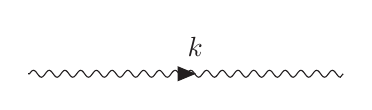
\begin{tikzpicture}[baseline]
			\begin{feynman}
				%% fig a
				\vertex (a1) at (0,0);
				\vertex[right =4cm  of a1] (a2);
				\node[above right =0.1cm and 1.9cm  of a1]{$k$};
				% 对各个顶点连线
				\diagram*{
				(a1) --[charged boson](a2),
				};
			\end{feynman}
		\end{tikzpicture}
	\end{minipage}
	 & \quad &
	\frac{i}{k^2-\mu^2}\left(\frac{k_\mu k_\nu}{\mu^2}-g_{\mu\nu}\right)
\end{align}

光子传播子(其中$\xi$是任意规范参数):\\
\begin{align}\label{equ:app.c.12}
	\begin{minipage}[c][5ex][c]{8em}
		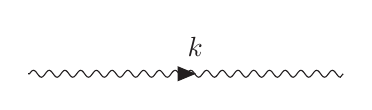
\begin{tikzpicture}[baseline]
			\begin{feynman}
				%% fig a
				\vertex (a1) at (0,0);
				\vertex[right =4cm  of a1] (a2);
				\node[above right =0.1cm and 1.9cm  of a1]{$k$};
				% 对各个顶点连线
				\diagram*{
				(a1) --[charged boson](a2),
				};
			\end{feynman}
		\end{tikzpicture}
	\end{minipage}
	 & \quad &
	\frac{i}{k^2}\left[(1-\xi)\frac{k_\mu k_\nu}{\mu^2}-g_{\mu\nu}\right]
\end{align}

矢量玻色子-费米子顶点:\\
\begin{align}\label{equ:app.c.13}
	\begin{minipage}[c][8ex][c]{8em}
		\begin{tikzpicture}[baseline]
			\begin{feynman}
				%% fig a
				\vertex (a1) at (0,0);
				\vertex[right =4cm  of a1] (a2);
				\vertex[above right =0cm and 2cm  of a1] (a3);
				\vertex[above right =1.5cm and 2cm  of a1] (a4);
				\node[above right =1.1cm and 2.1cm  of a1]{$\mu$};
				% 对各个顶点连线
				\diagram*{
				(a1) --[fermion]  (a3)--[fermion](a2),
				(a3)--[photon](a4)
				};
			\end{feynman}
		\end{tikzpicture}
	\end{minipage}
	 & \quad &
	ie\gamma^\mu
\end{align}

初始外线矢量玻色子:
\begin{equation}\label{equ:app.c.14}
	\varepsilon_\mu(k)
\end{equation}

终止外线矢量玻色子:
\begin{equation}\label{equ:app.c.15}
	\varepsilon_\mu(k)^\ast
\end{equation}

\section{非阿贝尔规范理论}

规范玻色子传播子:\\
\begin{align}\label{equ:app.c.16}
	\begin{minipage}[c][5ex][c]{8em}
		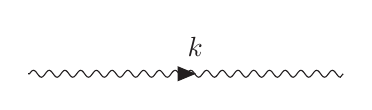
\begin{tikzpicture}[baseline]
			\begin{feynman}
				%% fig a
				\vertex (a1) at (0,0);
				\vertex[right =4cm  of a1] (a2);
				\node[above right =0.1cm and 1.9cm  of a1]{$k$};
				% 对各个顶点连线
				\diagram*{
				(a1) --[charged boson](a2),
				};
			\end{feynman}
		\end{tikzpicture}
	\end{minipage}
	 & \quad &
	\frac{i}{k^2}\left[(1-\xi)\frac{k_\mu k_\nu}
	{\mu^2}-g_{\mu\nu}\right]\delta_{ab}
\end{align}

鬼场传播子:\\
\begin{align}\label{equ:app.c.17}
	\begin{minipage}[c][5ex][c]{8em}
		\begin{tikzpicture}
			\begin{feynman}
				%% fig a
				\vertex (a1) at (0,0);
				\vertex[right =4cm  of a1] (a2);
				\node[above right =0.1cm and 1.9cm  of a1]{$k$};
				% 对各个顶点连线
				\diagram*{
					{ [edge=charged scalar]		(a1) --  (a2),
						},
				};
			\end{feynman}
		\end{tikzpicture}
	\end{minipage}
	 & \quad &
	\frac{i}{k^2}\delta_{ab}
\end{align}

规范玻色子间三次相互作用:\\
\begin{align}\label{equ:app.c.18}
	\begin{minipage}[c][15ex][c]{10em}
		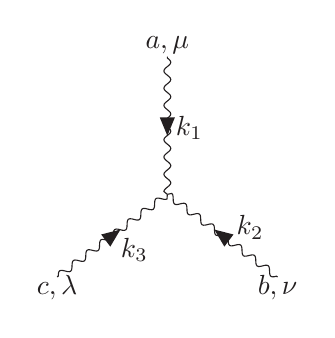
\begin{tikzpicture}[x=0.7cm,y=0.7cm]
			\begin{feynman}
				%% fig a
				\vertex (a1) at (0,0);
				\vertex[above right =2.5 and 0  of a1] (a2);
				\node [above right =2.7 and 0  of a1,anchor=center] {$a, \mu$};
				\node [above right =1.2 and 0.4  of a1,anchor=center] {$k_1$};
				\vertex[above right =-1.5 and -2 of a1](a3);
				\node[above right =-1.7 and 2 of a1,anchor=center]{$b,\nu$};
				\node[above right =-.6 and 1.5 of a1,anchor=center] {$k_2$};
				\node[above right =-1.7 and -2 of a1,anchor=center] {$c, \lambda$};
				\node[above right =-1 and -.6 of a1,anchor=center] {$k_3$};
				\vertex[above right =-1.5 and 2 of a1](a4);
				% 对各个顶点连线
				\diagram*{
				(a2) --[charged boson](a1),
				(a3) --[charged boson](a1),
				(a4) --[charged boson](a1),
				};
			\end{feynman}
		\end{tikzpicture}
	\end{minipage}
	 & \quad &
	gf^{abc}[g_{\mu\nu}(k_1-k_2)_\lambda+g_{\nu\lambda}(k_2-k_3)_\mu
	+g_{\lambda\mu}(k_3-k_1)_\nu]
\end{align}

规范玻色子间四次相互作用:\\
\begin{tabular}{ccc}
	\begin{minipage}[c][25ex][c]{10em}
		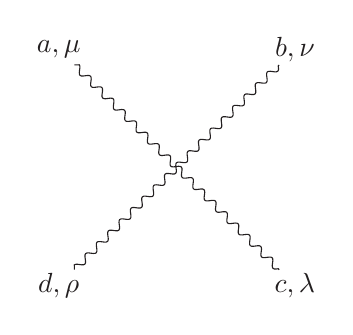
\begin{tikzpicture}[baseline]
			\begin{feynman}
				%% fig a
				\vertex[dot] (a1) at (0,0);
				\vertex[above right =1.3 and 1.3  of a1] (a2); % 右上
				\node [above right =1.5 and 1.5  of a1,anchor=center] {$b, \nu$};
				\vertex[above right =-1.3 and 1.3  of a1] (a3); % 右下
				\node [above right =-1.5 and 1.5  of a1,anchor=center] {$c, \lambda$};
				\vertex[above right =1.3 and -1.3  of a1] (a4); %左上
				\node [above right =1.5 and -1.5  of a1,anchor=center] {$a, \mu$};
				\vertex[above right =-1.3 and -1.3  of a1] (a5); %左下
				\node [above right =-1.5 and -1.5  of a1,anchor=center] {$d, \rho$};
				% 对各个顶点连线
				\diagram*{
					{ [edge=photon]	(a2) --  (a5),(a3) --  (a4),
						},
				};
			\end{feynman}
		\end{tikzpicture}
	\end{minipage}
	 & \quad &
	\begin{minipage}[c][25ex][c]{18em}
		\begin{align}\label{equ:app.c.19}
			-ig^2[f^{abe}f^{cde}(g_{\mu\lambda}g_{\nu\rho}
			-g_{\mu\rho}g_{\nu\lambda}) \notag     \\
			+f^{ade}f^{cbe}(g_{\mu\lambda}
			g_{\nu\rho}-g_{\mu\nu}g_{\rho\lambda}) \\
			+f^{ace}f^{bde}(g_{\mu\nu}g_{\lambda\rho}
			-g_{\mu\rho}g_{\nu\lambda})] \notag
		\end{align}
	\end{minipage}
\end{tabular}

规范玻色子与鬼场耦合:\\
\begin{align}\label{equ:app.c.20}
	\begin{minipage}[c][18ex][c]{9em}
		\begin{tikzpicture}[baseline]
			\begin{feynman}
				%% fig a
				\vertex[dot] (a1) at (0,0);
				\vertex[above right =1.3 and 0  of a1] (a2); % 上
				\node [above right =1.5 and 0  of a1,anchor=center] {$c, \mu$};
				\vertex[above right =-.9 and 2  of a1] (a4); % 右下
				\node [above right =-.8 and 1  of a1,anchor=center] {$b$};
				\vertex[above right =-1.3 and -1.7  of a1] (a5); %左下
				\node [above right =-.9 and -.7  of a1,anchor=center] {$a$};
				\node [above right =-.6 and -1.2  of a1,anchor=center] {$p$};
				% 对各个顶点连线
				\diagram*{
				(a2) --[photon] (a1),(a4) --[charged scalar](a1),(a5) --[anti charged scalar]  (a1),
				};
			\end{feynman}
		\end{tikzpicture}
	\end{minipage}
	 & \quad &
	gf^{abc}p^\mu
\end{align}


\section{散射截面和衰变率}

给出过程$p_1+p_2\rightarrow k_1+k_2+\cdots+k_n$的费曼振幅
$\mathfrak{M}$,其微分散射截面为
\begin{equation}\label{equ:app.c.21}
	d\sigma=\frac{1}{|\vec{v}_1-\vec{v}_2|\mathfrak{E}(p_1)\mathfrak{E}(p_2)}
	\frac{d^3k_1}{(2\pi)^3\mathfrak{E}(k_1)}\cdots
	\frac{d^3k_n}{(2\pi)^3\mathfrak{E}(k_n)}(2\pi)^4
	\delta^{(4)}(p_1+p_2-\sum_{i=1}^nk_i)|\mathfrak{M}|^2
\end{equation}
这里$\vec{v}_1$和$\vec{v}_2$表示入射粒子的速度。
玻色子的能量因子$\mathfrak{E}(p)=2\sqrt{\vec{p}^2+m^2}$
和费米子的能量因子$\mathfrak{E}(p)=\sqrt{\vec{p}^2+m^2}/m$
来自\ref{chap:I.8}和\ref{chap:II.2}中产生湮灭算符的不同的归一化。

对质量为$M$的粒子的衰变,其在自身静止参照系下微分衰变率为
\begin{equation}\label{equ:app.c.22}
	d\Gamma=\frac{1}{2M}\frac{d^3k_1}{(2\pi)^3\mathfrak{E}(k_1)}
	\cdots\frac{d^3k_n}{(2\pi)^3\mathfrak{E}(k_n)}(2\pi)^4
	\delta^{(4)}(P-\sum_{i=1}^nk_i)|\mathfrak{M}|^2
\end{equation}

\end{document}